\section{AM (Amplitudenmodulation) \schaum{43}}
	Bei der Amplitudenmodulation ist die Amplitude des Trägersignals $A(t)$ linear vom Nachrichtensignal $m(t)$ abhängig. Daher wird die Amplitudenmodulation oftmals als lineare Modulation bezeichnet.\\ 
	\begin{tabular}{l l l}
		Trägersignal & carrier & $A(t)=A_c \cdot \cos(\omega_c t)$ \\
		Nachrichtensignal & message & $m(t)$, oft normiert als $m_n(t)$: $|m_n(t)| < 1$  \\
		Moduliertes Signal & & $ x(t) \sim m(t) $ \\
	\end{tabular}\\
	
	\textbf{AM im Frequenzbereich}:\\
	Durch die Multiplikation eines Signals $x(t)$ mit $\cos(\omega_0 t)$ verschiebt sich dessen Spetrum $X(\omega)$ nach $\pm \omega_0$, konkret:\\
		$x(t) \cdot \cos(\omega_0 t) \FT \frac{1}{2} X(\omega - \omega_0) + \frac{1}{2} X(\omega + \omega_0) $

	%TODO: Klassifizierung von AM

\subsection{DSB(-SC): Doppelseitenband (Double-Sideband)-AM \schaum{44}} \label{am_dsb_modulation}
	Bei der Doppelseitenband-Amplitudenmodulation ist das untere Seitenband (Lower Sideband) sowie das obere Seitenband (Upper Sideband) präsent. Da der Träger im Spektrum nicht präsent ist, ist bei dieser Art von AM auch von \textbf{DSB-SC (Double-Sideband Suppressed Carrier)} die Rede. \\ 
	\begin{tabular}{l l l}
		\textbf{Bandbreite}: & $B_{X(\omega)} = 2 \cdot B_{M(\omega)}$ & \\
		\textbf{Leistung}: & $P_{DSB} = P_m \cdot \frac{A_c^2}{2}$ & \\
	\end{tabular}

\subsubsection{Modulation DSB}
\begin{minipage}[c][2.7cm][t]{6.5cm}
    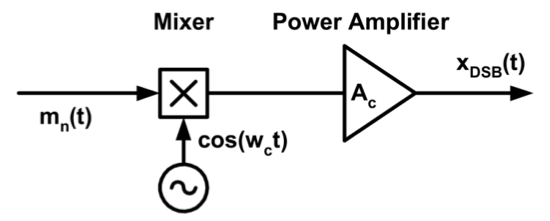
\includegraphics[width=6cm]{bilder/am_dsb_modulation.png}
\end{minipage}
\begin{minipage}[c][2.7cm][t]{11.5cm}
Bei der Doppelseitenband AM wird das Nachrichtensignal mit dem sinusförmigen Trägersignal
multipliziert, wodurch sich gemäss dem Modulationssatz folgendes Spektrum ergibt. \\
	$ \boxed{x_{_{DSB}}(t) = m_n(t) \: A_c \: \cos(w_c t)} \: \laplace 
	\: X_{DSB} = \frac{A_c}{2}M(\omega - \omega_c) + \frac{A_c}{2}M(\omega + \omega_c)$
\end{minipage}

\begin{minipage}[c]{9cm}
    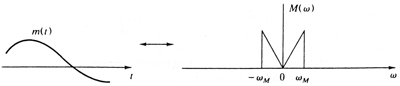
\includegraphics[width=9cm]{bilder/am_dsb_nachrichtensignal.png}
\end{minipage}
$\xrightarrow{\text{DSB-AM}}$
\begin{minipage}[c]{9cm}
    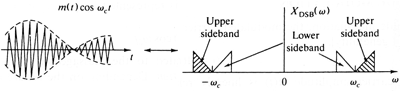
\includegraphics[width=9cm]{bilder/am_dsb_spektrum.png}
\end{minipage}

\subsubsection{Demodulation DSB} 
\label{am_dsb_demodulation}
\begin{minipage}[t][2.3cm][c]{6.5cm}
    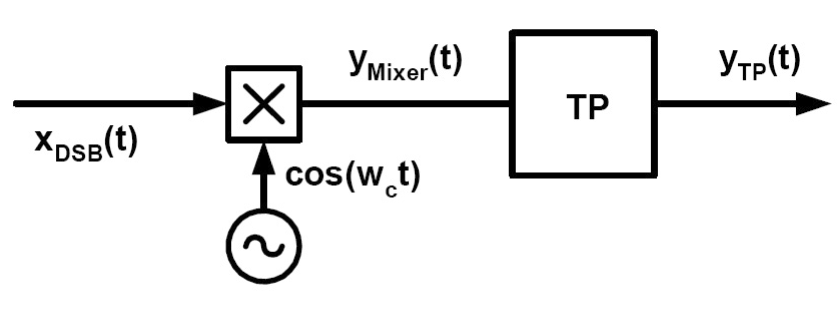
\includegraphics[width=6cm]{bilder/am_dsb_demodulation}
\end{minipage}
\begin{minipage}[t][2.3cm][c]{11.5cm}
	Das DSB-Signal wird mit einem sogenannten \textbf{synchronen Demodulator} oder \textbf{koharänten
	Demodulator} zurückgewonnen. Hierbei wird das DSB-Signal mit dem lokalen Träger
	multipliziert und anschliessend das Nachrichtensignal mittels einem Tiefpassfilter rausgefiltert.
	\\ 
\end{minipage} \\

\begin{tabular}{l l l}
	$y_{_{Mixer}}(t) = x_{_{DSB}}(t) \cdot \cos(\omega_ct)$ & $\laplace$ &  
	$Y_{_{Mixer}}(\omega) = \frac{1}{2} A_c M(\omega) + \frac{1}{4} A_c (M(\omega-2\omega_c) + M(\omega+2\omega_c))$ \\
	$y_{_{TP}}(t) = T_{LPF}[y_{_{Mixer}}(t)] $&$ \laplace $&$ Y_{TP}(\omega) = \frac{1}{2}A_cM(\omega)$ \\
\end{tabular} \\ \\

	Weicht die Frequenz oder die Phase des Demodulators $x_{osc}$ von deren des Modulators ab, 
	so ergeben sich Abschwächungen im demodulierten Nachrichtensignal.\\
\textbf{Auswirkungen einer Phasenabweichung um $\varphi$:} $\boxed{y_{TP}(t) = \frac{1}{2} m(t) \cos(\varphi)} $ mit $x_{osc} = \cos(\omega_c t + \varphi)$ \\
\textbf{Auswirkungen einer Frequenzabweichung um $\Delta \omega$:} $ \boxed{y_{TP}(t) =
\frac{1}{2} m(t) \cos(\Delta \omega t)}$ mit $x_{osc} = \cos((\omega_c + \Delta \omega)t )$ \\

\newpage

\subsection{AM: Gewöhnliche(Ordinary)-AM \schaum{45}}
	Die gewöhnliche AM wird generiert, indem man vor der Multiplikation mit dem Trägersignal noch ein DC-Anteil dazugibt.

\subsubsection{Modulation OAM}
	$\boxed{x_{_{AM}}(t) = (1 + \mu \cdot m_n(t)) \cdot A_C \cdot  \cos(\omega_c t)}
	\; \laplace \; X_{AM}(\omega) = \frac{1}{2} \mu A_c M(\omega - \omega_c) + 
	\frac{1}{2} \mu A_c M(\omega + \omega_c) + \pi A_c [\delta (\omega - \omega_c) + 
	\delta (\omega + \omega_c)] $ \\
	$ \text{mit} \qquad m(t) \; \laplace \; M(\omega) $ \\
	
\begin{minipage}[]{9cm}
	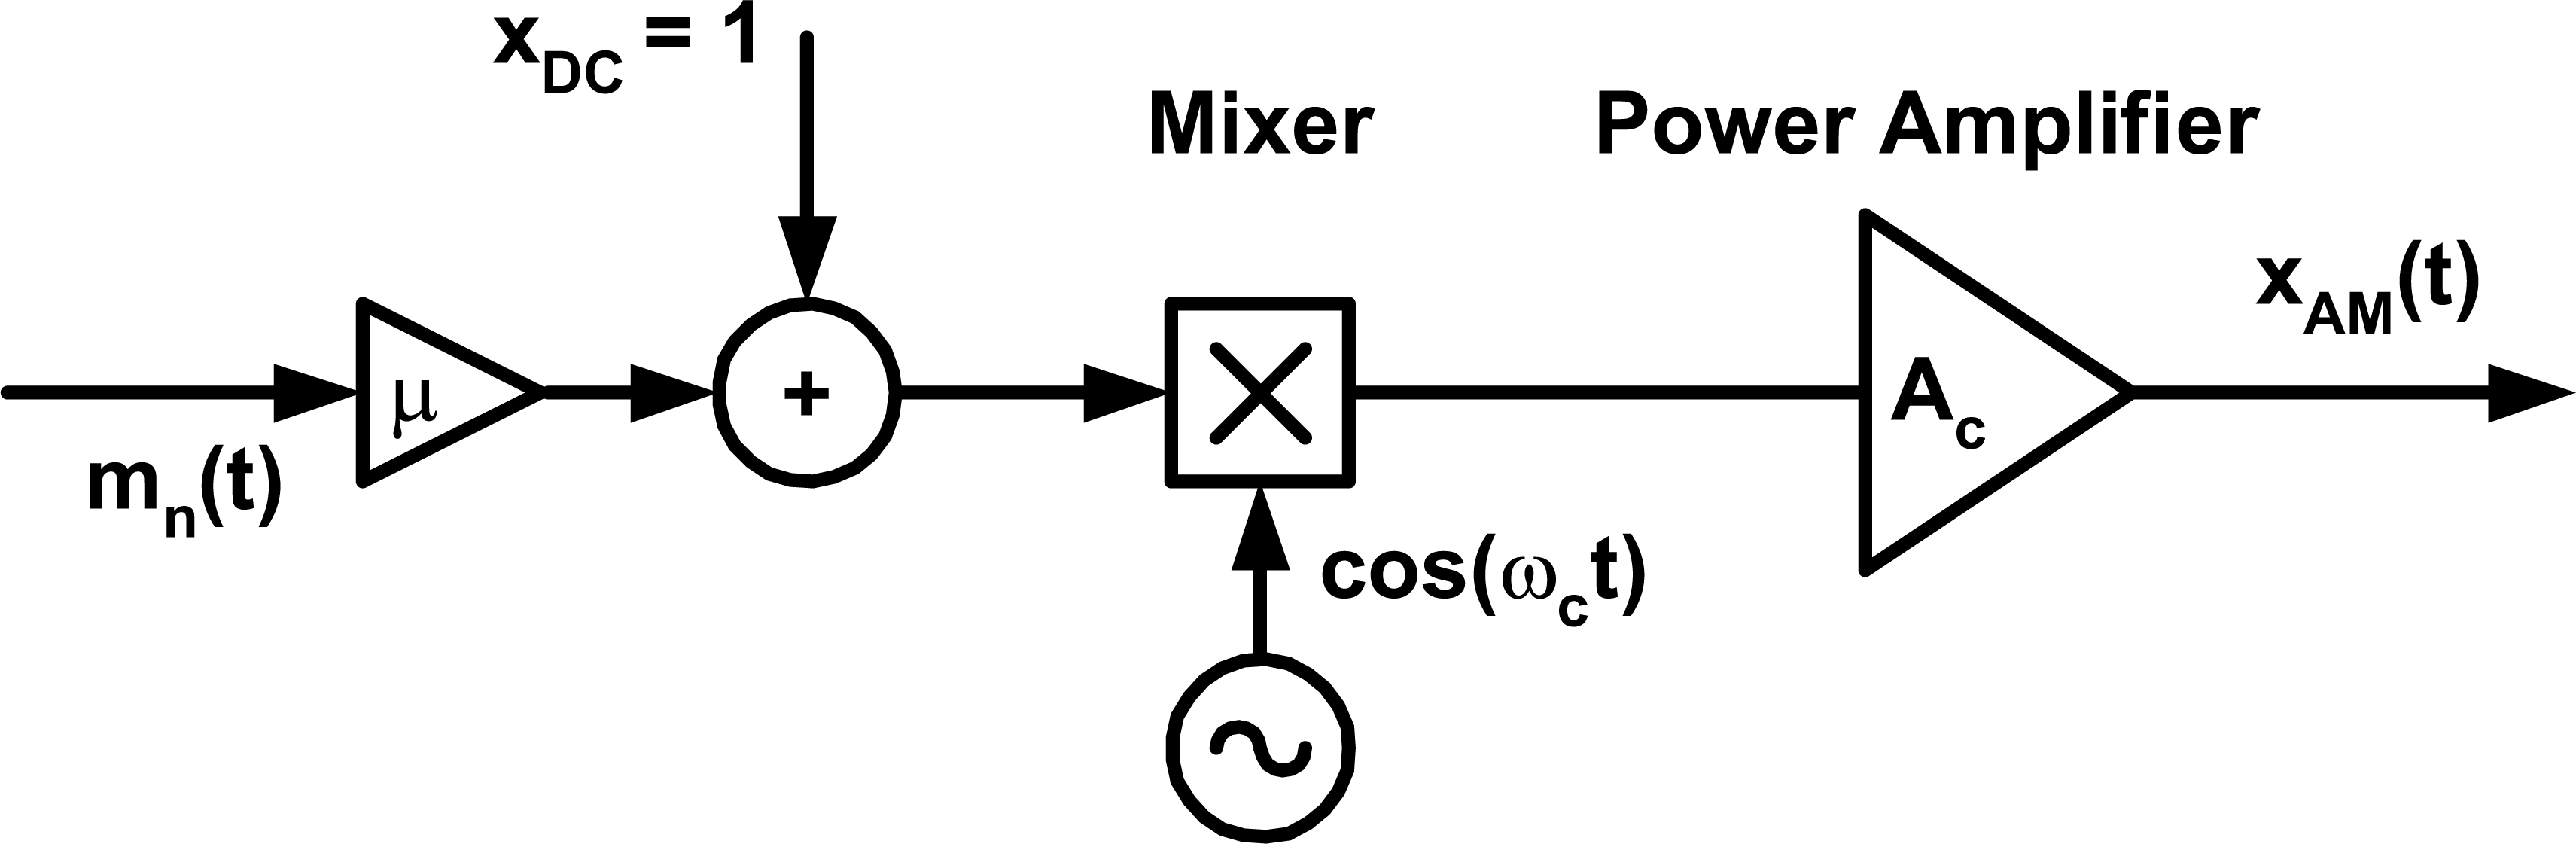
\includegraphics[width=7cm]{bilder/am_oam_modulation.png}
\end{minipage}
\begin{minipage}[]{9cm}
    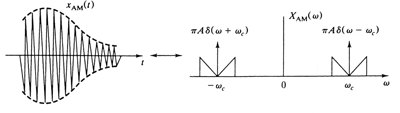
\includegraphics[width=9cm]{bilder/am_oam_spektrum.png}
\end{minipage}\\

Die Bandbreite bleibt gleich wie bei DSB-AM, jedoch befindet sich nun ein grosser Teil der
Signalleistung im Träger. \\
Diese Art von AM hat sich v.a. in füheren Zeiten durchgesetzt, weil die Demodulation mit sehr
wenig Aufwand realisiert werden kann. 

\subsubsection{Demodulation OAM}
\textbf{Mit Enveloppen Detektor}  \\
Der Enveloppen Detektor braucht nur drei Bauteile, der Schaltungsaufwand ist entsprechend gering.\\ \\
\begin{minipage}{7cm}	
      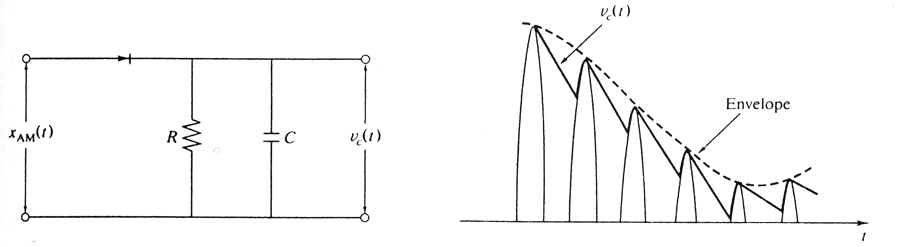
\includegraphics[width=7cm]{bilder/am_oam_enveloppeDetektor.png}
\end{minipage}
\begin{minipage}{11cm}
Damit der Envelope Detektor korrekt funktioniert müssen R und C korrekt gewählt werden, es gilt: \\
\framebox{$RC \leq \frac{\sqrt{1 - \mu^2}}{\omega_m \mu}$}  was gleichbedeutend ist mit: 
$\frac{1}{RC} \geq \omega_m \frac{\mu \cdot \sin(\omega_m t_0)}{1+\mu\cdot\cos(\omega_mt_0)}$ \\ \\
In der Praxis genügt jedoch meist das Erfüllen der Bedingung $B_m < \frac{1}{RC} \ll f_c$,
wobei es sich bei $B_m$ um die Bandbreite des Nachrichtensignals handelt. 
\end{minipage} \\

\textbf{Mit kohärentem (synchronen) Demodulator}\\
Ordinary AM kann auch mit dem kohärenten Demodulator demoduliert werden:
$y(t) = \frac12 (A + m(t)) = \frac12 m(t) + \frac12 A$ mit nachfolgendem
seriellem Kondensator (Hochpass zum Filtern des DC-Anteils).


\subsubsection{Modulationsindex \schaum{46}}
Der Modulationsindex $\mu$ ist für AM wie folgt definiert: $ \boxed{\mu = \dfrac{|min\{m(t)\}|}{A_c} = \dfrac{A_m}{A_c}}$\\

Um eine Demodulation mit dem Envelope-Detektor zu ermöglichen, muss die Bedingung 
\textbf{$\mu \leq 1$} erfüllt sein. \\
Ist dies nicht der Fall (\textbf{$\mu > 1$}) so spricht man von einer \textbf{Übermodulation} oder
einem  \textbf{übermodulierten Träger}, was in einer Envelope-Verzerrung resultiert. \\
Anbei zwei Fälle zur Veranschaulichung dieser Problematik: Links ($\mu \ll 1$), Rechts ($\mu > 1
\rightarrow $ Übermodulation).

\begin{minipage}[t][2.3cm][c]{9.5cm}
	\begin{center}
      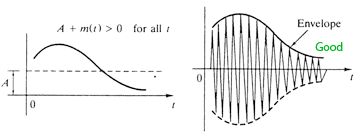
\includegraphics[width=8cm]{bilder/am_oam_enveloppeGood.png}
	\end{center}
\end{minipage}
\begin{minipage}[t][2.3cm][c]{9.5cm}
    \begin{center}
    	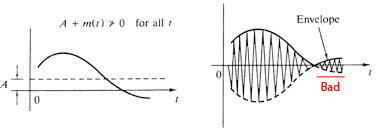
\includegraphics[width=8cm]{bilder/am_oam_enveloppeBad.png}
	\end{center}
\end{minipage}

\subsubsection{Effizienz / Wirkungsgrad OAM \schaum{55-3.4}}
Unter der Effizienz $ \eta $ der gewöhnlichen AM versteht man das Verhältnis von der Signalleistung
$P_s$ der beiden Seitenbänder zur Gesamtleistung $P_t$ des AM-Signals. $P_c$ entspricht der Leistung des Trägersignals und $P_m$ der des modulierenden Nachrichtensignals.

\[ P_t = \frac{1}{2}A_c^2(1 + \mu^2 \cdot P_m) =  \frac{A_c^2}{2} + \frac{\mu^2 A_c^2}{2}\cdot P_m = P_c + P_s  \quad 
\Longrightarrow 
\quad \eta = \frac{P_s}{P_t} = \frac{\frac{1}{2}A_c^2 \mu^2 P_m}{\frac{1}{2}A_c^2(1 + \mu^2 P_m)} = \frac{\mu^2 \cdot P_m}{1 + \mu^2 \cdot P_m}\]

Die maximale Effizienz (bei $\mu = 100\% $ und $P_m = 1/2$) beträgt nur gerade $ \eta = 33\% $. 

\subsection{SSB: Einseitenband (Single-Sideband)-AM \schaum{47}}
	\begin{minipage}{14cm}
		Sowohl Gewöhnliche AM als auch DSB verschwenden Bandbreite, weil diese immer beide Seitenbänder übermitteln. \\ 
		Ist dies nicht der Fall - wird somit \textbf{nur ein Seitenband} übertragen - so spricht man von 	Einseitenband-AM. Deren Vorteil liegt in der Reduktion der Bandbreite, was aber auch den Nachteil 	- Die Komplexität der Implementation - mit sich bringt.
	\end{minipage}
	\begin{minipage}{5cm}
		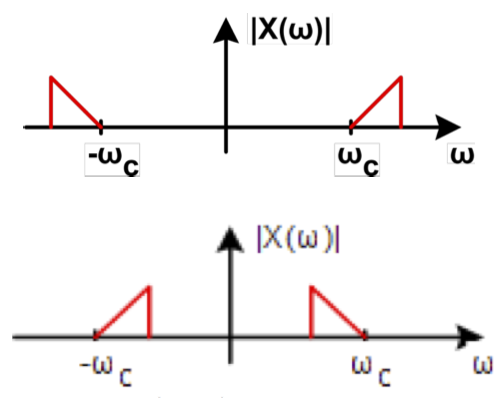
\includegraphics[width = 4cm]{bilder/am_ssb_spektrum}
	\end{minipage}

\subsubsection{Modulation SSB \schaum{57-3.7}}
\textbf{Phasenverschiebung }  \\
\begin{minipage}[t][3.7cm][c]{7.0cm}
    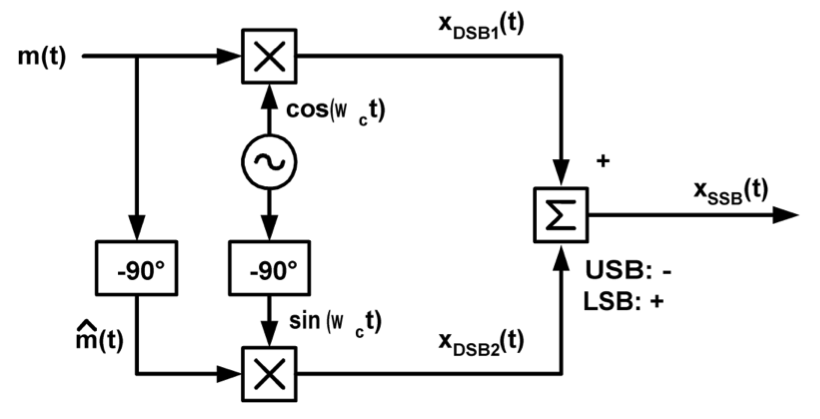
\includegraphics[width=6.5cm]{bilder/am_ssb_modulationPhasenshifter.png}
\end{minipage}
\begin{minipage}[t][3.7cm][c]{11cm}	
	Eine Möglichkeit ein SSB-Signal zu generieren ist mit Hilfe von $ - 90^{\circ} $-Phasenschiebern , {\small siehe
	\ref{lti_quadratur} Quadraturfilter/Hilbertransformation (S. \pageref{lti_quadratur})}.
	Phasenschiebung auf $m(t)$ angewendet: \\
	$\hspace*{0.5cm}\hat{m}(t) \; \laplace \; -\im \sgn(\omega) M(\omega) = -\im M_+(\omega) + \im M_-(\omega)$ \\
	Nachdem das Signal \"ahnlich der DSB-AM moduliert wurde, kann durch das entsprechende Vorzeichen des phasenverschobenen Signals das entsprechende Seitenband ausgewählt werden:\\ 
	$+$: Lower Sideband; \qquad $-$: Upper Sideband
	
	Die Amplitude des SSB-Signals ist im Spektrum \textbf{gleich hoch} wie die des
	Nachrichtensignals.
\end{minipage}\\

\textbf{Filtermethode} \\
\begin{minipage}[t][2cm][c]{5.5cm}
    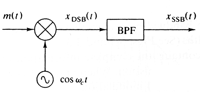
\includegraphics[width=5cm]{bilder/am_ssb_modulationFilter.png}
\end{minipage}
\begin{minipage}[t][2cm][c]{12.5cm}	
	Hierbei wird ein DSB-Signal mit einem Hoch- oder Tiefpass gefiltert, sodass ein SSB-Signal
	resultiert. Diese Methode ist in der \textbf{Praxis unüblich}, da sehr steile Filter benötigt
	werden.\\
	Die Amplitude des SSB-Signals ist im Spektrum \textbf{halb so hoch} wie die des
	Nachrichtensignals.
\end{minipage}

\subsubsection{Demodulation SSB}
Zur Demodulation kann die gleiche Phasenschieber-Schaltung wie zur Modulation verwendet
werden. Die Signale werden jedoch immer addiert, nie subtrahiert. \\
Die Demodulation kann auch mit dem koheränten Demodulator (siehe \ref{am_dsb_modulation} DSB-AM) erfolgen, dabei entspricht\\
$Y_{LPF}(\omega) = \frac{1}{4}M(\omega)$ \\


\subsection{VSB: Restseitenband (Vestigial-Sideband)-AM}
	\begin{minipage}{12cm}
		Restseitenband-AM ist sozusagen die praktische Realisierung der Frequenzdiskriminierungsmethode bei
		SSB. \\
		Vorteil: extreme Anforderungen an Filter-Flankensteilheit entfallen.\\
		Nachteil: ben\"otigt ca. 1.25 x Bandbreite von SSB
	\end{minipage}
	\begin{minipage}{5cm}
		\begin{center}
		    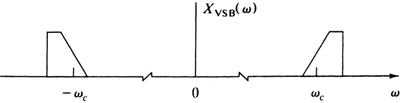
\includegraphics[width=5cm]{bilder/am_vsb_spektrum.png}
		\end{center}
	\end{minipage}
	
	\subsubsection{Modulation VSB}
		\begin{minipage}[t][2.2cm][c]{5.5cm}
    		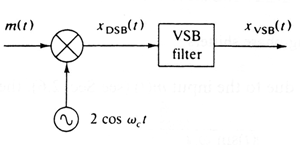
\includegraphics[width=5cm]{bilder/am_vsb_modulator.png}
		\end{minipage}
		\begin{minipage}[t][2.2cm][c]{12.5cm}	
			\begin{itemize}
				\item Filter d\"ampft eines der Seitenbänder zu Restseitenband
				\item Filterkurve läuft antisymmetrisch bzgl. der Trägerfrequenz: \\
				$H(\omega +
				\omega_c) + H(\omega - \omega_c) = const$ für $|\omega| \leq |\omega_m|_{max}$
				\item Schlussendlich resultiert das VSB-Singal  mit etwa 1.25-facher Bandbreite von SSB. $ \qquad  W_{VSB} \approx 1.25 \cdot W_{SSB} $
			\end{itemize}
		\end{minipage}


\subsubsection{Demodulation VSB}
	Auch diese Art von AM kann mit einem kohärenten Demodulator demoduliert werden. Dabei ist die antisymmetrie der Filterkurve für eine verzerrungsfreie Demodulation erforderlich.
	Auch hier entspricht $Y_{LPF}(\omega) = \frac{1}{4}M(\omega)$


\subsection{QAM: Quadratur-AM}
	\begin{minipage}{12cm}
		Hierbei werden zwei orthogonale Träger ($\sin, \cos$) verwendet, sodass zwei Nachrichtensignale zusammen übertragen werden können. Dies ist zwar technisch aufwendiger, jedoch wird die Bandbreite doppelt genutzt. \\
		Bei der Demodulation muss darauf geachtet werden, dass der Demodulator synchronisiert ist. Ist dies nicht der Fall, so kann sich bei grösserer Phasenabweichung das andere Nachrichtensignal ``einschleichen''.
	\end{minipage}
	\begin{minipage}{7cm}
		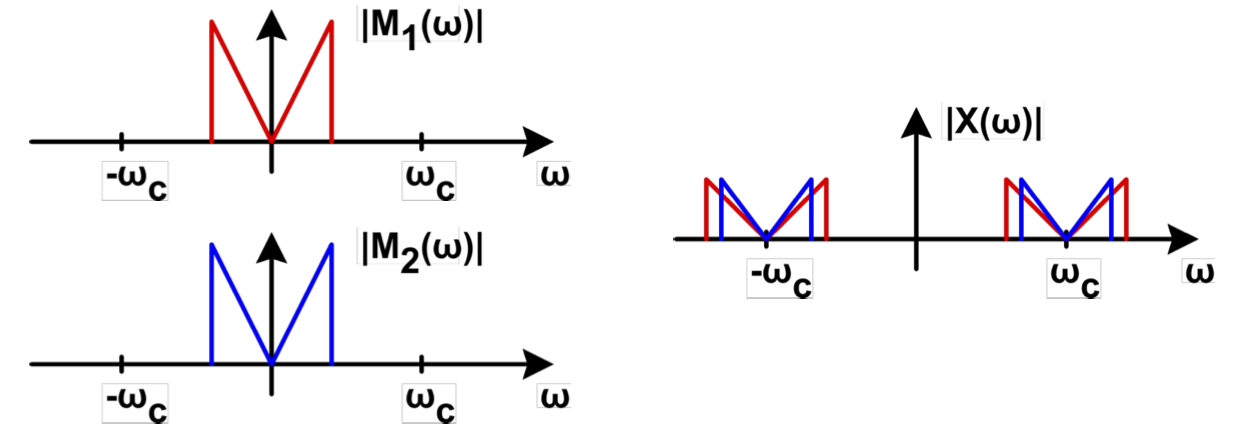
\includegraphics[width=7cm]{bilder/am_qam_spektrum.png}
	\end{minipage}
	\begin{center}
    	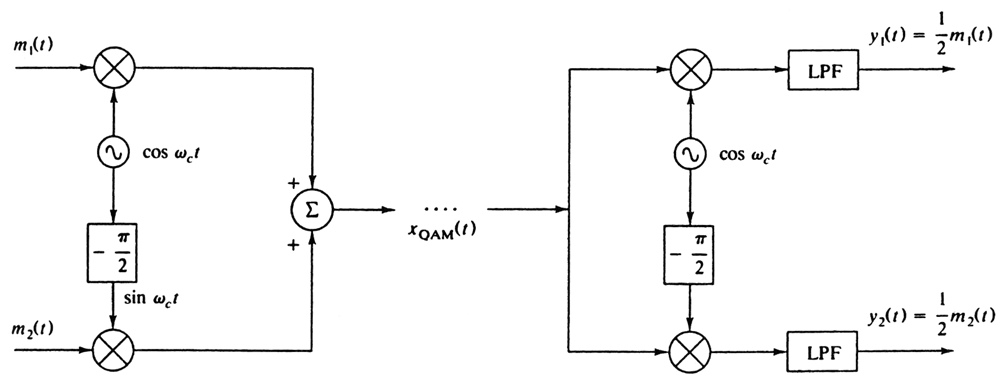
\includegraphics[width=14cm]{bilder/am_qam_modulatorDemodulator.png}
	\end{center}
